\section{GRB models}
\label{sec:GRB_models}
Most GRB analysis within IceCube use information from observed GRBs to look
for neutrino clusters in time and space correlated to the detected GRBs.
This strategy has the obvious advantage of reducing the neutrino background to
achieve higher significance per GRB observation. However, due to the limited
Field of View of the satellites there will be many GRBs that stay undetected.
Furthermore, one is biased by the detection sensitivity of the satellites.

In this analysis, a GRB population is assumed based on theoretical work and
extrapolation based on data from Swift and other satellites. The redshift and
luminosity functions are extracted.
The neutrino luminosity function is assumed to have the same shape and is
shifted in energy by an efficiency factor $\epsilon$ (see section 
\ref{sec:norm2HESE}).
%  to calculate their
% expected signal in IceCube.
The different population models under consideration are discussed in this
chapter.

The main analysis has been done based on the luminosity function and GRB rate
density calculated by Wanderman and Piran (\ref{ssec:WP}). 
The other models presented here were considered to examine the dependency on
the assumed model.

\subsection{Cosmology}
The following cosmological definitions are used in the calculations of the 
following chapters.

\textbf{Differential co-moving shell volume} 
\begin{equation}
dV = 4 \pi D_H \frac{(1+z)^2D_a^2(z)}{K(z)}dz
\end{equation}
\textbf{Hubble distance}
\begin{equation}
 D_H = \frac{c}{H_0} = 3000 h^{-1}\text{Mpc}
\end{equation}
\textbf{Angular distance}
\begin{equation}
 D_a(z) = (1+z)^{-2} D_l(z)
\end{equation}
\textbf{Parameters} 
\begin{itemize}
  \item  $K(z) = \sqrt{\Omega_m (1 + z)^3 + \Omega_{\Lambda}}$
 \item $h=0.7$
 \item $\Omega_m = 0.3$
 \item $\Omega_\Lambda$
\end{itemize}

\subsection{Wanderman Piran}
\label{ssec:WP}
Wanderman and Piran \cite{WP} extracted a GRB distribution in redshift and
luminosity using GRB data up to 2009 applying detection efficiencies for
both the detection in $\gamma$- rays and a following determination of the host
redshift, i.e., the redshift of the GRB. 

The differential co-moving rate of bursts (fig. \ref{fig:GRB_rate_density}) at a
redshift $z$ is
\begin{equation}
 R(z) = \frac{R_{\text{GRB}}(z)}{(1+z)} \frac{dV(z)}{dz}
 \label{eq:Rz}
\end{equation}
$dV(z)/dz$ is the differential co-moving shell volume 
and the factor $(1+z)^{-1}$ reflects the cosmological time dilation.
$R_{\text{GRB}}$ is fitted to data with the result (Fig \ref{fig:RGRB})
\begin{equation}
\label{eq:R_z}
    R_{\text{GRB}}(z) = \begin{cases}
                        \rho_0 \cdot (1 + z)^{n_1} & z \leq z_1 \\
			 \rho_0 \cdot (1 + z_1)^{n_1 - n_2}(1 + z)^{n_2} & z >
z_1
                        \end{cases}
\end{equation}
with
$n_1= 2.07$, $n_2=-1.36$, $z_1=3.11$ and the local rate $\rho_0=1.25
\text{Gpc}^{-3} \text{yr}^{-1}$.

% 1.25 \cdot 10^{-9} \cdot \text{Mpc}^{-3} \cdot \text{yr}^{-1}$

\begin{figure}[h]
\centering
 \captionsetup{width=.9\textwidth}
%  \captionsetup{margin=0pt}
\subfloat[Derived RGRB function (WP)\label{fig:RGRB}]{%
 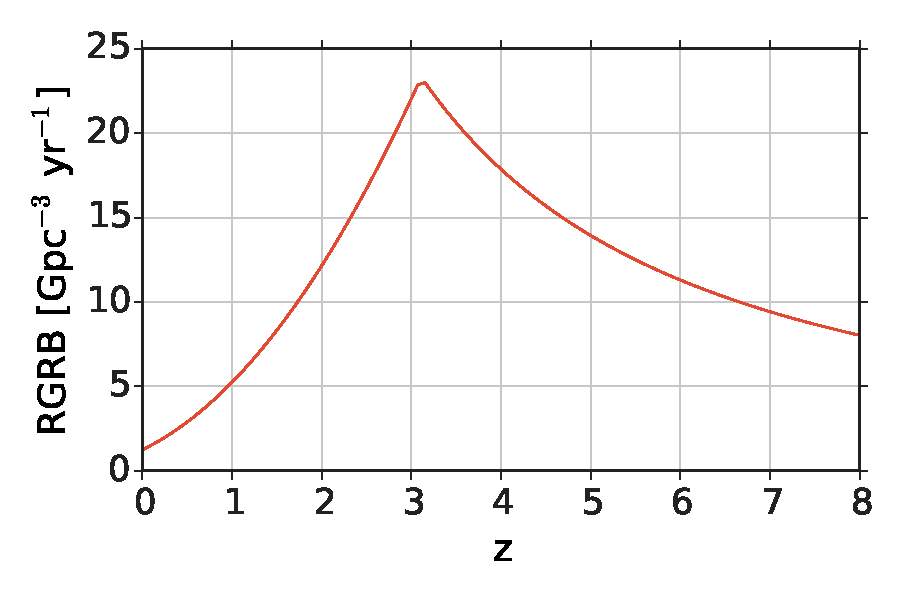
\includegraphics[width=0.45\textwidth]{fig/RGRB_WP.pdf}}
 \subfloat[Differential co-moving rate\label{fig:GRB_rate_density}]{%
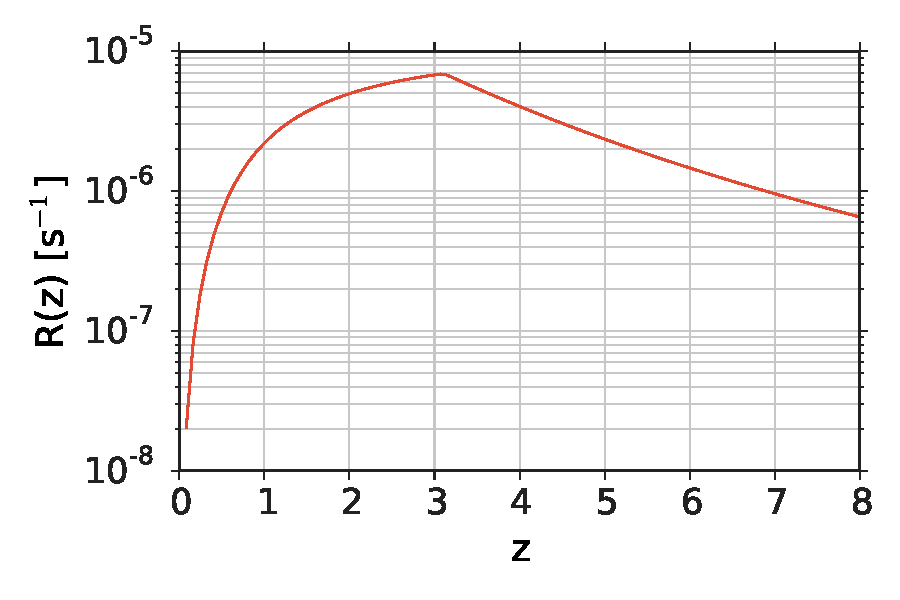
\includegraphics[width=0.45\textwidth]{fig/Rz_WP.pdf}}
\caption{The distribution of GRBs over the redshift displaying the derived RGRB 
function and the differential co-moving rate.}
\end{figure}




The peak $\gamma$-luminosity at the source
$L_{\text{Peak}}$ (Fig. \ref{fig:Lpeak})  is determined to follow
\begin{equation}
\label{eq:Phi_L}
 \Phi(L_{\text{Peak}}) = \begin{cases}
      \left(\frac{L}{L_{*}} \right)^{-\alpha} &  L < L_{*} \\
      \left(\frac{L}{L_{*}} \right)^{-\beta}  &  L > L_{*}
     \end{cases}
\end{equation}
in which $\text{log}_{10}L_{*}=52.53 \text{ erg / s}$ is the break luminosity
and $\alpha=0.17$ and $\beta=1.44$ are the spectral indices (Table
\ref{tab:grb_model_params}).
No redshift evolution of the luminosity is assumed.
\begin{figure}[h]
% \begin{minipage}{\textwidth}
 \captionsetup{width=.6\textwidth}
 \centering
%  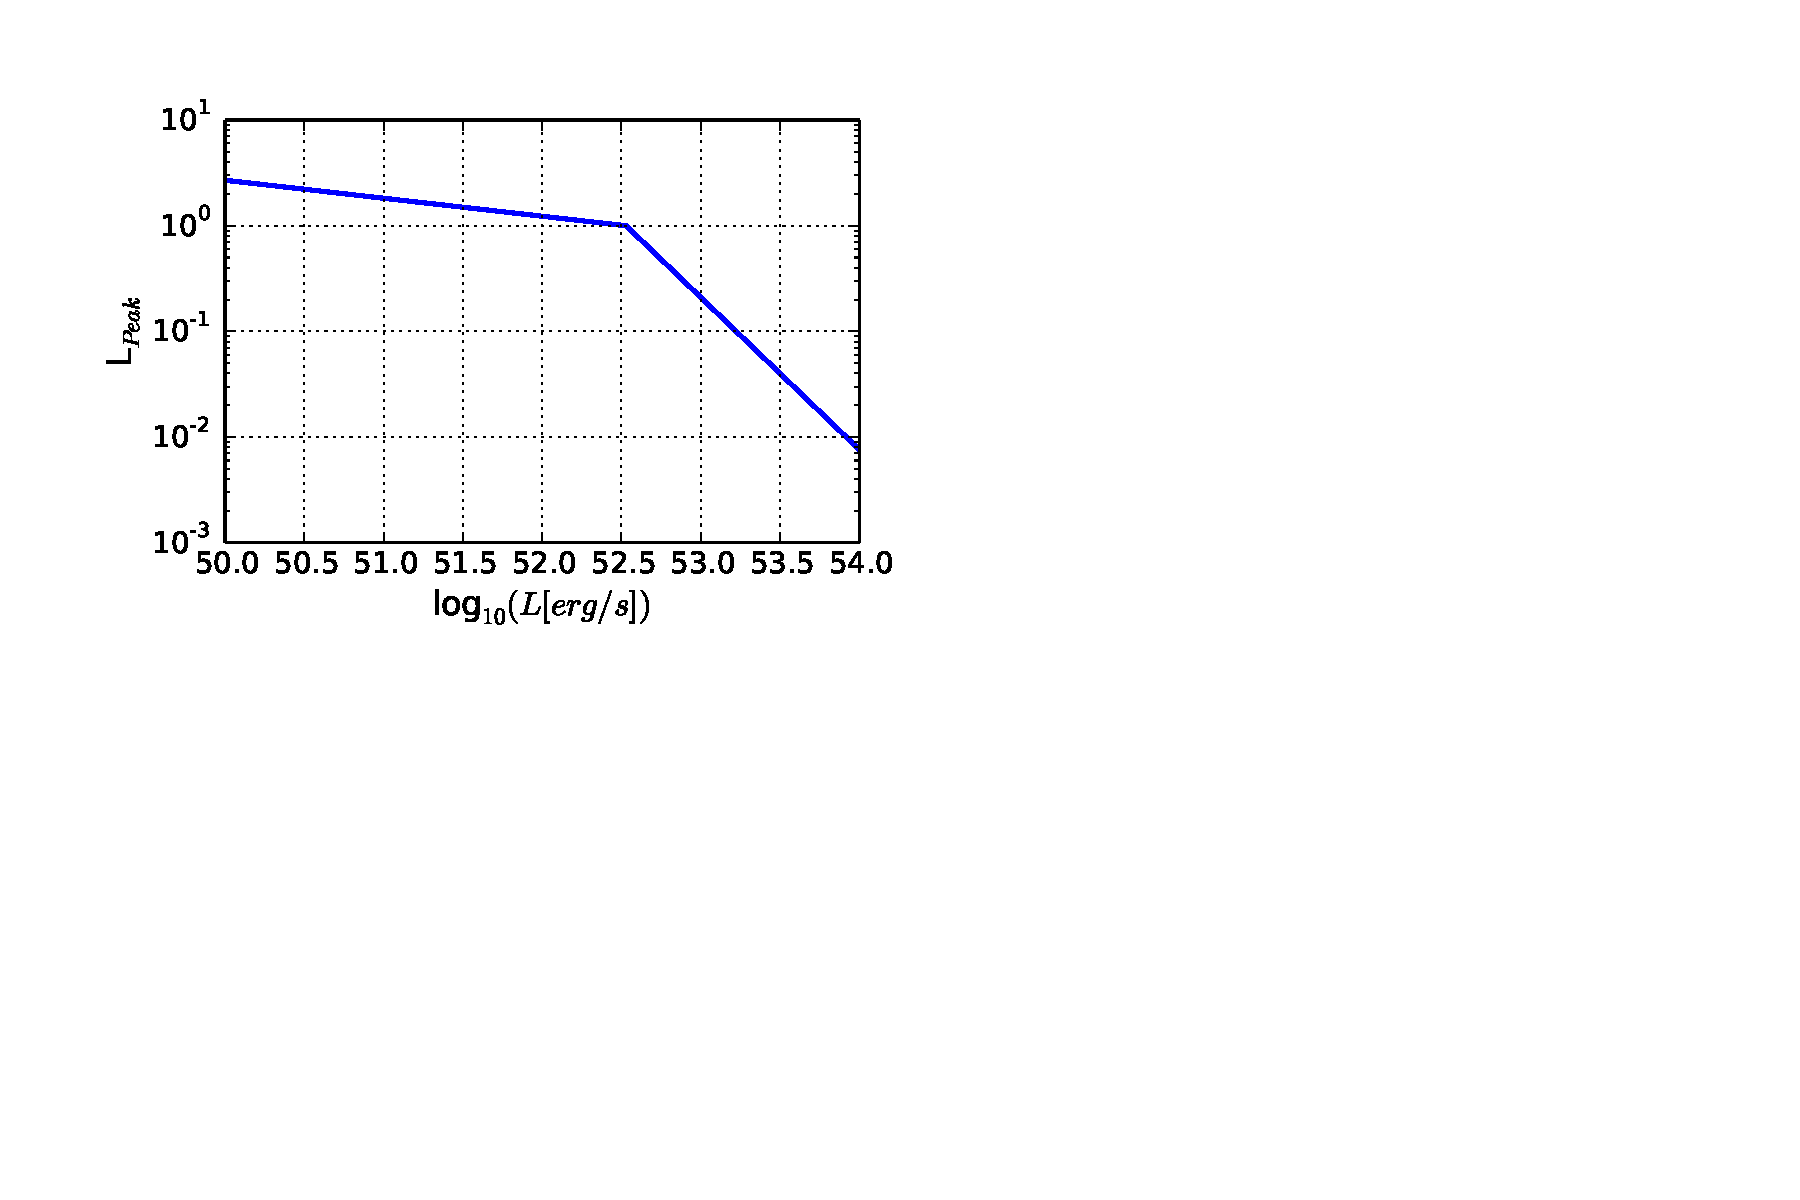
\includegraphics{fig/Lpeak.pdf}
 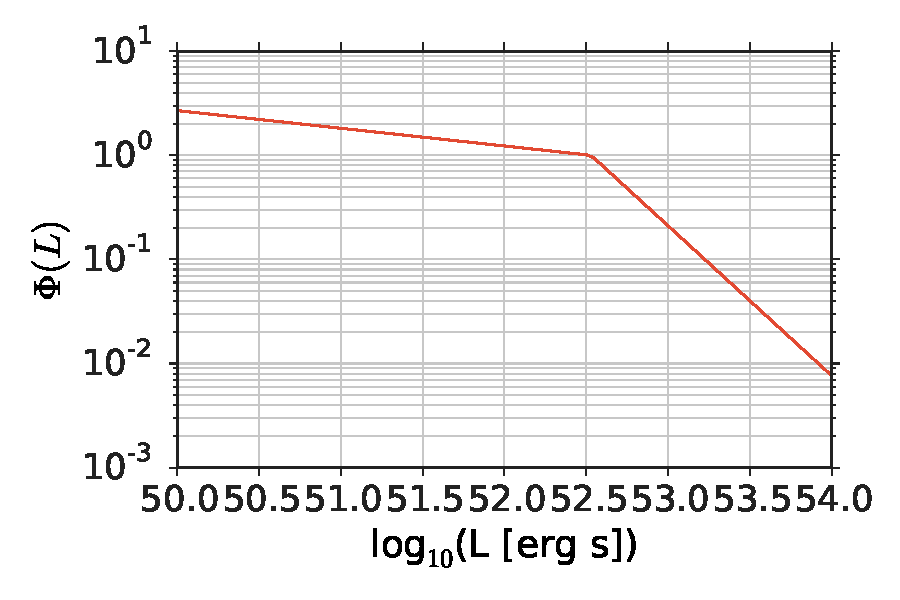
\includegraphics[width=0.6\textwidth]{fig/Lpeak_wp.pdf}
 \caption{The luminosity function derived in the WP model. (deleted this figure 
and use the one including HC?)}
 \label{fig:Lpeak}
% \end{minipage}
\end{figure}
\subsection{Howell Coward}
\begin{table}[h]
  \centering
  \begin{tabular}{l||c|c|c|c|c|c|c|c|c}
    Model & log$_{10}\left(L_* \left[ \text{erg} \text{ s}^{-1} \right] \right)$
& $\alpha$ & $\beta$ & $\rho_0 \left[\text{Gpc}^{-3} \text{ yr}^{-1} \right]$ &
$z_1$ & $n_1$ & $n_2$ & $N_\text{GRB}$ \\
    \hline
    WP & 52.53 & 0.17 & 1.44 & 1.25 & 3.11 & 2.07 & -1.36 & 9082.83\\
%     HC 1 & 51.9 & 0.95 & 2.59 & 0.48 & 3.6 & 2.1 & -0.7 & 4791.97\\
    HC & 51.7 & 0.13 & 2.42 & 0.48 & 3.6 & 2.1 & -0.7 & 4791.97\\
  \end{tabular}
  \caption{Fit parameters to the luminosity functions and redshift
distributions of the tested models.}
  \label{tab:grb_model_params}
\end{table}
There is a more recent work \cite{HC} by Howell, Coward, Stratta,
Gendre and Zhou basing the redshift distribution on
the same general shape as Wanderman Piran and testing various luminosity 
functions. For purposes of
readability it will be called Howell-Coward or HC-model. 
One of the tested luminosity functions
will be compared to the model by Wanderman and
Piran (WP). 
%They are designated HC1 and HC2.

Similarly to Wanderman and Piran, the luminosity is assumed to not evolve
with redshift in their main work.
The same functions as in WP are used for redshift distribution (eq. 
\ref{eq:R_z}) and the
luminosity function (Eq. \ref{eq:Phi_L}), but different fit results
were obtained for the parameters (Table \ref{tab:grb_model_params}).

The considered luminosity range is with $\text{log}_{10} L_\text{Peak} \in
\left( 49, 54 \right)$ larger than in WP ($\text{log}_{10} L_\text{Peak} \in
\left( 50, 54 \right)$). The break peak luminosity is lower
than in WP transitioning into a harder slope towards higher luminosities (Fig.
\ref{fig:wp_hc_comp}). At lower luminosities the slopes of HC and WP are
quite similar (0.13, 0.17) leading to more low luminosity GRBs in HC due to the 
greater range.

% The redshift distribution in HC is shifted to smaller values of $R(z)$ as a
% smaller local rate and total number of GRBs is assumed (Table
% \ref{tab:grb_model_params}). 
The redshift distributions rise to the break redshift quite similarly although 
the break is at higher redshifts (3.6 compared to 3.11) for HC transitioning
into a slower decay at large $z$. The overall impact are more distant GRBs in
HC than in WP which should lead to a slight weakening of the limits.

\begin{figure}[ht]
% [htb] 
\subfloat[Luminosity functions\label{fig:wp_hc_comp_lum}]
{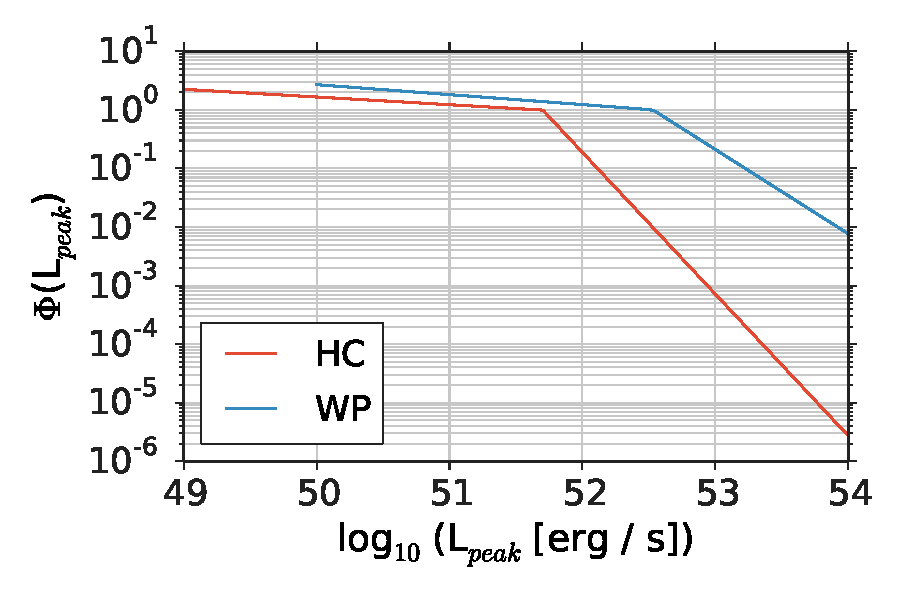
\includegraphics[width=0.48\textwidth]{fig/grb_models_lum_comp_L45.pdf}}
    \hfill
\subfloat[Redshift distributions\label{fig:wp_hc_comp_z}]
{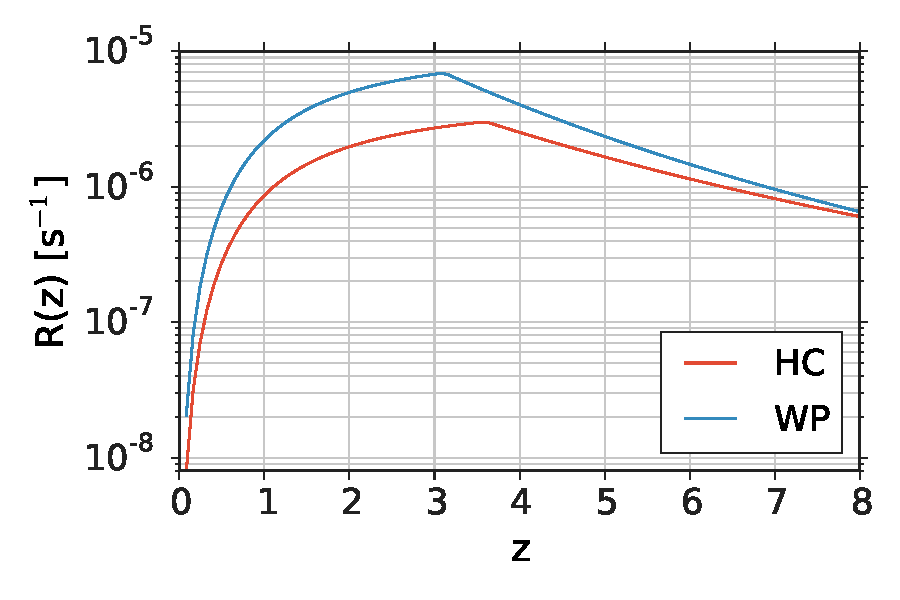
\includegraphics[width=0.48\textwidth]{fig/grb_models_redshift_comp.pdf}}
    \caption{The luminosity functions (left) from the
Wanderman-Piran model and two functions from the HC model on the left. The WP
only take into account luminosities in the range of $10^{50} - 10^{54}$ erg / s
which is reflected in the shorter blue line.\\
The redshift distributions (right) develop similar up to $z=3.11$ at which point
it breaks for the WP-model. The HC predicts more GRBs at higher redshift
values.}
\label{fig:wp_hc_comp}
\end{figure}


% While most of cases discussed in (reference ???) imply independentend luminosity
% and redshift, a correction is given to examine the influence of a possible
% evolution. This will be added at a later point as a third comparison model.
\subsection{Long low luminosity GRBs}
In recent years, IceCube has started to rule out the first optimistic GRB
neutrino emission models leading to new ideas as to possible neutrino emitters.
It has been proposed \cite{lowlumgrbs} that a high number of very low
luminosity GRBs exists that are difficult to detect in $\gamma$-rays, but could
produce most of the neutrinos expected from GRBs. In principle, the follow-up
analysis based on IceCube triggers can be an approach to examine these objects.
Thus, they are mentioned here briefly for the sake of completeness and future 
possible Follow-Up extensions. 

Unfortunately, these low luminosity GRBs are predicted to have a prompt
emission phase in the range of $10^3$ s. The follow-up program suppresses
background by allowing a maximal time difference of 100s between two events
reducing the sensitivity to very long GRBs at the same time. Therefore, they
have not been examined yet within this analysis but mentioned for the 
interested reader.

\subsection{Supernovae}
The models presented described GRB population models. However, the Optical 
Follow-Up is sensitive to all short ($O(10 \text{ s})$) transient neutrino 
sources. E.g. the simulation can be used to examine a population of core 
collapse Supernovae (SNe) as well. A model predicting high energy neutrinos 
from SNe \cite{AB} assumes a jet production withing the SN similar to the jets 
of 
the GRB fireball model. Due to the lack of energy, they do not penetrate the 
stellar envelope and are therefore invisible to the telescopes 
observing the electromagnetic signal. In contrast, neutrinos would escape the 
SN and could possibly be detected within IceCube. The exact mechanism and 
resulting predicted spectrum is not important for this analysis as we assume a 
population of sources and attribute to them a spectrum that reproduces the 
measured HESE flux.
%Nora s work

SNe follow the star formation rate which, in first order, can be approximated 
by the Wanderman Piran redshift distribution. However, the luminosity function 
differs quite a bit by not showing the big variations in luminosity that are 
observed for GRBs. Instead, the luminosity function is assumed to follow a 
Gaussian curve in logarithmic space with a width of 0.4 orders of magnitudes 
corresponding to a width of one astronomical magnitude. A comparison to the WP 
luminosity function is shown in Figure \ref{fig:lum_SN}. The mean luminosity is 
chosen at random and will be later adjusted to create the expected neutrino 
flux.
% (Section ???).


\begin{figure}
 \centering
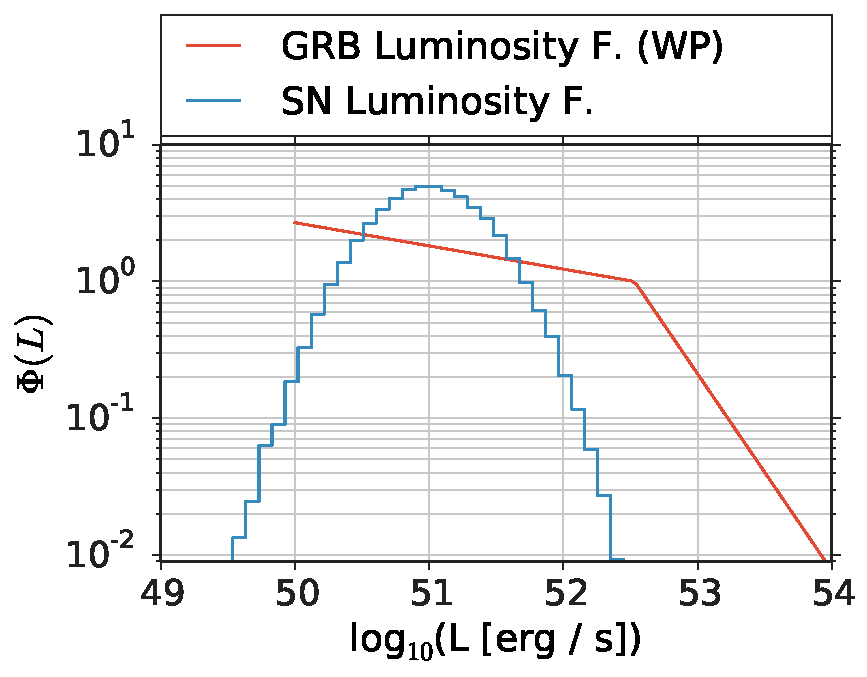
\includegraphics[width=0.65\textwidth]{fig/Lpeak_wp_SN.pdf}
\caption{}
\label{fig:lum_SN}
\end{figure}


\subsection{T90}
\begin{figure}[ht]
\centering
 \captionsetup{width=.68\textwidth}
{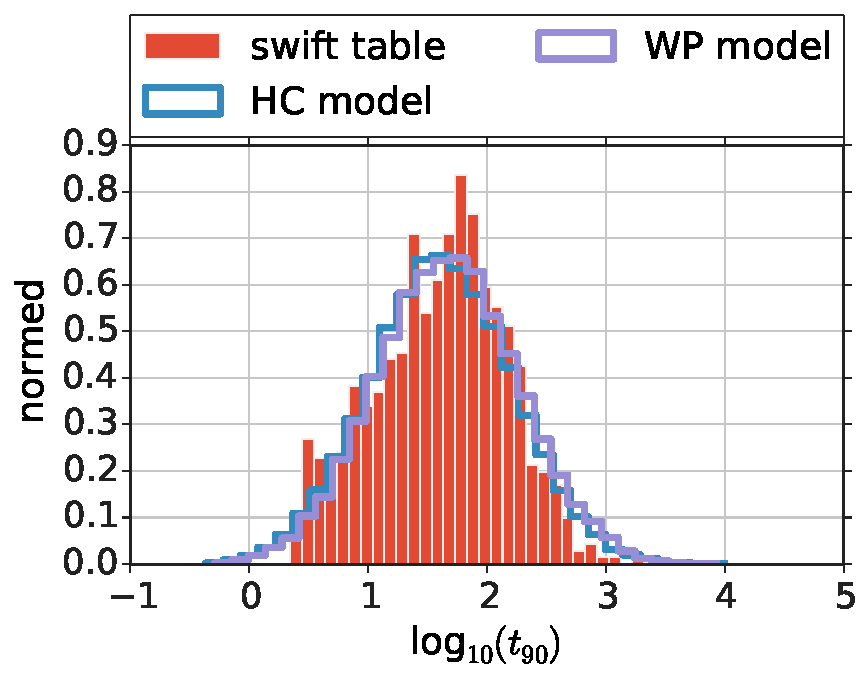
\includegraphics[width=0.68\textwidth]{fig/t90earth.pdf}}
    \caption{The $t_{90}$ distributions at earth based on data extracted from
the Swift database (reference ???) and the drawn distributions based on
$t_{90}$ values drawn at source and folded with the redshift distributions.}
\label{fig:t90earth}
\end{figure}
Ninety percent of the detectable $\gamma$-ray flux is received between a
time intervall called $t_{90}$. Reference (???) lists values for most GRBs.
The extracted values for long GRBs are displayed in figure \ref{fig:t90earth}. 

In the GRB Toy Monte Carlo $t_{90}$ values will be drawn at source (marked with
$\hat{}$ ) to
calculate the total energy output according to
\begin{equation}
 P\left(\hat{t}_{90}\right) = a \cdot \text{exp} \left( -
\frac{\left(\hat{t}_{90} -
b \right)^2}{2 c^2} \right).
\label{eq:t90dist}
\end{equation}
It will be folded with the drawn
redshift to calculate the $t_{90}$ pervieved at earth.
\begin{equation}
 t_{90} = \hat{t}_{90} \cdot \left( 1 + z \right)
\label{eq:t90earth}
\end{equation}
The $t_{90}$ distributions for the WP and HC models are displayed in figure
\ref{fig:t90earth} as well.



%table with parameters a,b,c
% \subsection{comparison}